\section{Results I: the CSI 300 through the white box}\label{sec:results-china}

\subsection{The lagging paradox in the data}
\Cref{tab:lagging} confirms \cref{sec:lagging} on all nineteen series. A 60-lag linear model fitted
to price levels by least squares has coefficients summing to $0.994$--$1.003$ and its forecast is
correlated with the previous close at $0.9993$ or more: it \emph{is} a random walk with estimation
noise. Its out-of-sample price RMSE exceeds the random walk's on every series, by $0.6\%$ (US
T-note) to $7.8\%$ (CSI~300 ETF), as \cref{prop:bound} and the cost of estimating 61 coefficients
predict. The differenced directional accuracy of the random walk equals sign persistence exactly and
lies between $0.44$ and $0.50$, which is why price-level models routinely report ``directional
accuracy below a coin flip''. None of these numbers measures forecasting skill.

\subsection{In-sample estimates}
\Cref{tab:csi300_params} reports the SMoE for CSI~300 over January 2005--June 2024 ($n=4{,}613$).
There are three main findings.

\emph{The mixture is strongly supported.} The likelihood ratio against the single-regime Gaussian
with the same covariates is $330.6$ for 18 additional parameters and BIC improves by 179
(\cref{tab:csi300_lik}). AIC ranks the SMoE first among the nested family; BIC prefers the more
parsimonious LSTAR, which shares the trend/reversal experts but drops the crisis expert and two gate
covariates.

\emph{Volatility is the regime variable; momentum and drawdown are not.} The robust Wald test that
all gate slopes are zero (SMoE against the constant-weight MAR) rejects at any conventional level
($W=70.8$, 6 df). Decomposing it, volatility enters the gate ($W=46.2$, 2 df, $p<10^{-9}$) whereas
60-day momentum ($p=0.14$) and drawdown ($p=0.14$) do not (\cref{tab:csi300_wald}). The trend expert's
weight falls with volatility ($\hat\gamma=-1.03$, $z=-6.4$): in calm markets two thirds of the
probability mass sits in the trend regime, and it drains towards the other experts as volatility rises
(\cref{fig:gate_curves}).

\emph{Semantic labels and estimated signs disagree, and the disagreement is informative.} The trend expert loads on
120-day momentum ($\hat\beta=0.106$, $z=3.8$), as its label suggests. The ``reversal'' expert,
however, has a \emph{positive} coefficient on the scaled one-day return ($0.278$, $z=2.2$) and a
large variance: in the high-variance state, Chinese index returns continue rather than reverse. The
``crisis'' expert has a positive mean ($1.77\%$, $z=6.5$) and captures the rebound days that follow
sell-offs. We return to the cross-market pattern in \cref{sec:results-global}: in developed markets
the same expert has the negative sign of genuine short-term reversal.

\begin{figure}[t]\centering
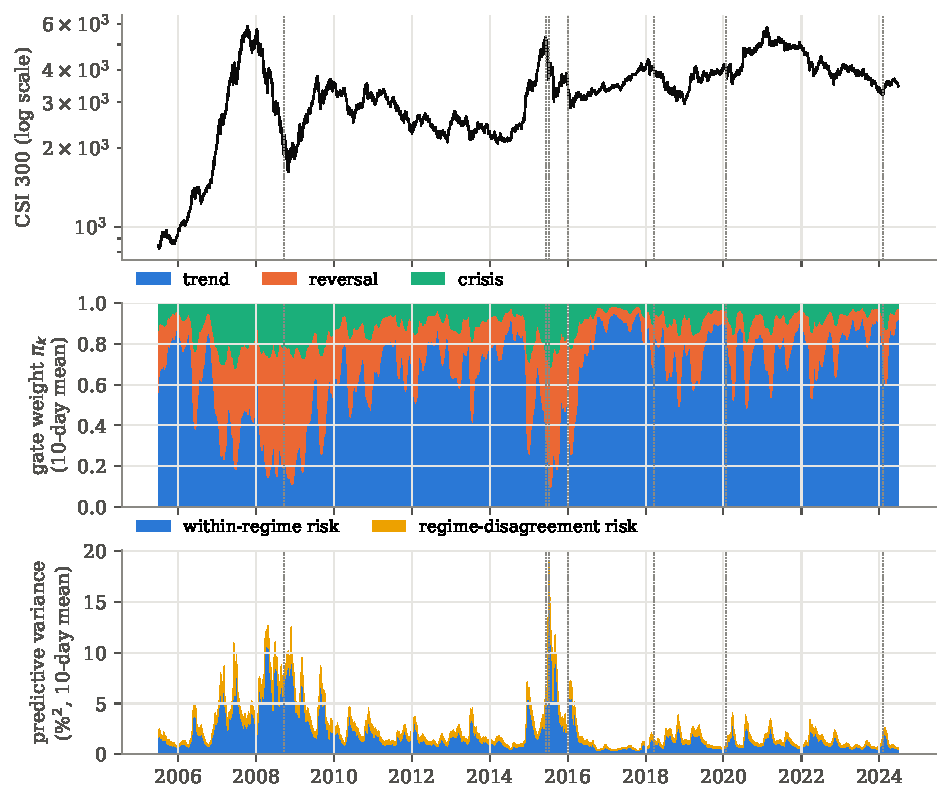
\includegraphics[width=\textwidth]{../results/figures/csi300_gates_risk.pdf}
\caption{CSI 300: price (top), SMoE gate probabilities (middle) and the decomposition of predictive
variance into within-regime and regime-disagreement risk (bottom), in sample. Dotted lines mark the
policy and market events of \cref{tab:events}.}\label{fig:gates}
\end{figure}

\begin{figure}[t]\centering
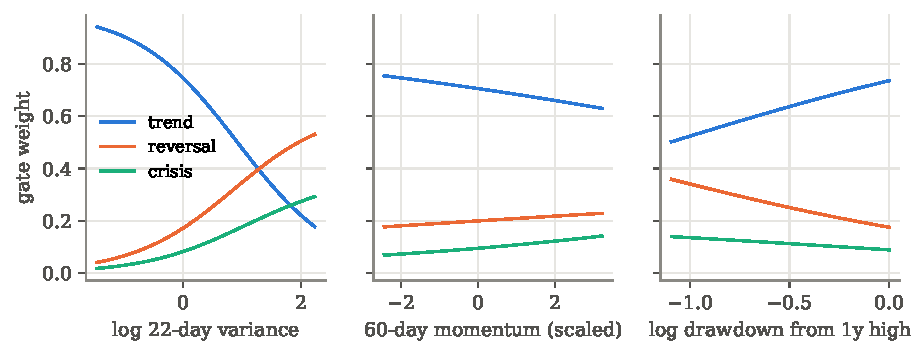
\includegraphics[width=\textwidth]{../results/figures/csi300_gate_curves.pdf}
\caption{Gate response curves for CSI 300: $\pi_k$ as a function of each state variable with the
others at their sample means. Only volatility moves the gate materially, matching the Wald tests.}
\label{fig:gate_curves}
\end{figure}

\subsection{Reading the forecasts}
\Cref{fig:whitebox} applies the closed forms of \cref{sec:whitebox} to the fitted CSI~300 model. The top
panel is the exact attribution \eqref{eq:attr} of the predictive mean to the three experts. The
short-horizon (``reversal'') and crisis experts carry large and opposite contributions that largely
cancel; in the 2008 and 2015 turmoil both widen to about half a percentage point a day. The predictive
\emph{mean} is therefore the small difference of two large regime-specific forecasts. This is a reason to
distrust any single point forecast of the daily return, and seeing it requires a mixture with explicit
components. The middle panel shows the probability of a rise, which exceeds one half on 64\% of
days but rarely departs from it by more than ten percentage points.

The bottom panel is the gate elasticity of the 1\% VaR with respect to the volatility state,
computed in closed form (\cref{app:derivations}). Through the gate alone (holding every expert's mean
and variance fixed) a one-standard-deviation rise in log volatility lowers the 1\% VaR by $0.58$
percentage points on average, with a 5--95\% range of $0.24$ to $0.83$. The effect is weakest in the
middle of the 2008 and 2015 crises, when the gate has already shifted most of its weight away from the
trend expert and has little left to move. Statements of this kind (exact, decomposed by channel and
state-dependent) are what we mean by a white box.

\begin{figure}[t]\centering
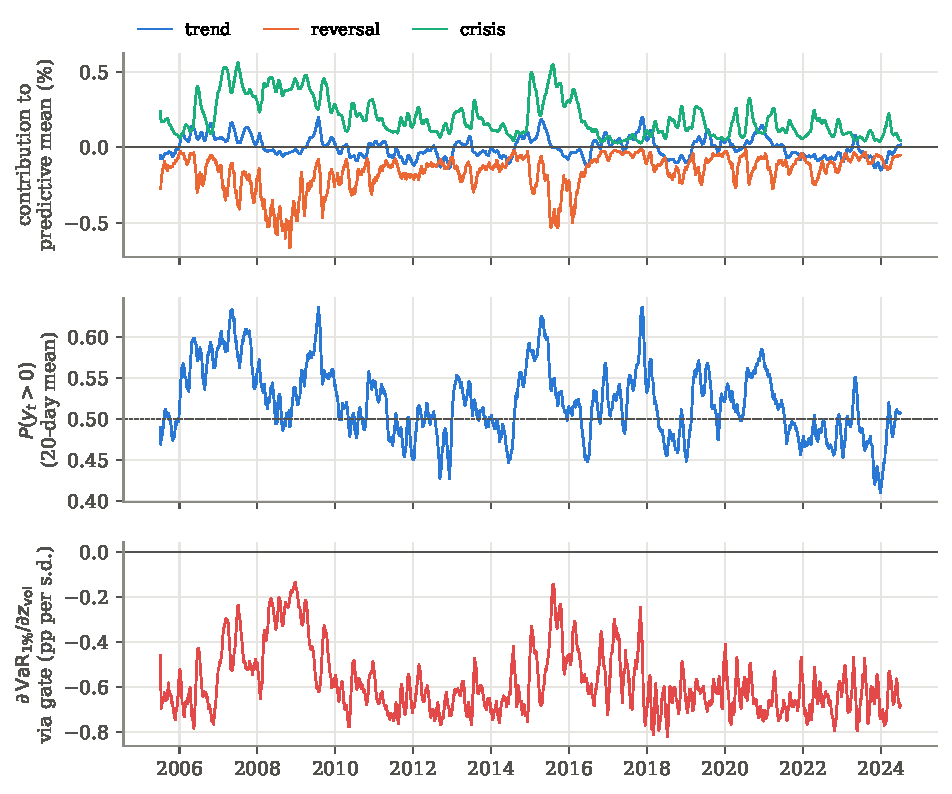
\includegraphics[width=\textwidth]{../results/figures/csi300_whitebox.pdf}
\caption{CSI 300 through the white box (in sample, 20-day averages). Top: exact attribution of the
predictive mean to the experts. Middle: probability of a rise. Bottom: closed-form gate elasticity of
the 1\% VaR with respect to the volatility state, in percentage points per standard deviation.}
\label{fig:whitebox}
\end{figure}

\subsection{Policy and market events}
Because the gate is a function of observables, its reading around known events is a falsifiable
description of what the model does. Around the start of the 2015 crash the 20-day average trend
weight halves (from $0.42$ to $0.21$) while the reversal and crisis weights rise; after the rescue
package of July 2015 the trend weight falls further to $0.11$. The circuit-breaker episode of January
2016 shows the same pattern in smaller magnitude. Two events move the gate the other way or not at
all: the 2018 tariff announcements coincided with a \emph{higher} trend weight (the sell-off was
gradual and low-volatility at first), and the 2008 stamp-duty cut left the weights unchanged. The
gate therefore responds to the change in volatility that an event brings; the headline itself does
not enter. This reading is available only because the gate is a known function of observables.

\subsection{Out-of-sample forecasts}
\Cref{tab:loss_NLL,tab:loss_CRPS,tab:loss_QLIKE,tab:loss_FZ5} report out-of-sample losses for all
models and assets relative to GARCH-$t$. For the Chinese equity series the SMoE ties with the GARCH
family. Its log-score difference from GARCH-$t$ is $-0.002$ (CSI~300), $-0.023$ (CSI~500), $+0.003$
(SSE~50) and $+0.004$ (ChiNext); for CSI~300 it is inside the 10\% model confidence set for all four
losses (MCS $p$-values $0.64$--$0.89$), together with the GARCH models, LSTAR and the deep SMoE.
Models that are \emph{excluded} for CSI~300 are equally informative: the historical Gaussian, the
Markov-switching regression and all three zero-shot foundation models under every loss, the boosted
model under every loss except CRPS, and the single-regime Gauss-HAR for log score.

The variance forecasts can be checked against realised variance from 5-minute data, which is a far
more precise proxy than squared returns. Against $\mathrm{RV}_t+r^2_{\text{overnight},t}$ the SMoE has
the highest Mincer--Zarnowitz $R^2$ of all models ($0.355$, versus $0.244$ for GARCH-$t$) and the
second-lowest MSE. On QLIKE four models are marginally better (LSTAR, Gauss-HAR, the boosted model
and the MAR, $0.293$--$0.299$ against $0.303$), all of which use the same range-based HAR variance
covariates (\cref{tab:rv}).


\begin{table}[!htbp]\centering\scriptsize
\caption{SMoE estimates for CSI 300, January 2005--June 2024}\label{tab:csi300_params}
\begin{adjustbox}{max width=\textwidth}
\begin{tabular}{lrrrrr}
\toprule
Parameter & Estimate & SE (sandwich) & SE (model) & $z$ & $p$\\
\midrule
\texttt{beta[trend]:const} & -0.000 & 0.029 & 0.029 & -0.002 & 0.998\\
\texttt{beta[trend]:mom20} & 0.011 & 0.025 & 0.024 & 0.426 & 0.670\\
\texttt{beta[trend]:mom120} & 0.106 & 0.028 & 0.027 & 3.809 & 0.000\\
\texttt{beta[reversal]:const} & -0.728 & 0.262 & 0.183 & -2.782 & 0.005\\
\texttt{beta[reversal]:rev1} & 0.278 & 0.126 & 0.120 & 2.208 & 0.027\\
\texttt{beta[reversal]:rev5} & 0.184 & 0.166 & 0.125 & 1.104 & 0.269\\
\texttt{beta[crisis]:const} & 1.773 & 0.272 & 0.229 & 6.516 & 0.000\\
\texttt{delta[trend]:const} & -0.219 & 0.120 & 0.093 & -1.833 & 0.067\\
\texttt{delta[trend]:lv1} & 0.054 & 0.070 & 0.064 & 0.769 & 0.442\\
\texttt{delta[trend]:lv5} & 0.012 & 0.115 & 0.104 & 0.107 & 0.915\\
\texttt{delta[trend]:lv22} & 0.376 & 0.115 & 0.108 & 3.270 & 0.001\\
\texttt{delta[reversal]:const} & 1.372 & 0.137 & 0.097 & 10.024 & 0.000\\
\texttt{delta[reversal]:lv1} & 0.226 & 0.087 & 0.088 & 2.591 & 0.010\\
\texttt{delta[reversal]:lv5} & 0.245 & 0.124 & 0.117 & 1.979 & 0.048\\
\texttt{delta[reversal]:lv22} & 0.159 & 0.116 & 0.102 & 1.372 & 0.170\\
\texttt{delta[crisis]:const} & -0.327 & 0.290 & 0.263 & -1.125 & 0.261\\
\texttt{delta[crisis]:lv1} & 0.422 & 0.187 & 0.209 & 2.254 & 0.024\\
\texttt{delta[crisis]:lv5} & 0.065 & 0.235 & 0.272 & 0.274 & 0.784\\
\texttt{delta[crisis]:lv22} & 0.331 & 0.206 & 0.225 & 1.603 & 0.109\\
\texttt{gamma[trend]:const} & 1.970 & 0.407 & 0.339 & 4.845 & 0.000\\
\texttt{gamma[trend]:g\_lvol} & -1.033 & 0.162 & 0.149 & -6.385 & 0.000\\
\texttt{gamma[trend]:g\_mom60} & -0.216 & 0.146 & 0.124 & -1.481 & 0.139\\
\texttt{gamma[trend]:g\_dd} & 0.154 & 0.141 & 0.129 & 1.091 & 0.275\\
\texttt{gamma[reversal]:const} & 0.725 & 0.481 & 0.362 & 1.505 & 0.132\\
\texttt{gamma[reversal]:g\_lvol} & -0.053 & 0.172 & 0.151 & -0.311 & 0.756\\
\texttt{gamma[reversal]:g\_mom60} & -0.112 & 0.203 & 0.157 & -0.549 & 0.583\\
\texttt{gamma[reversal]:g\_dd} & -0.049 & 0.156 & 0.125 & -0.316 & 0.752\\
\bottomrule
\end{tabular}
\end{adjustbox}
\par\smallskip\begin{minipage}{\textwidth}\footnotesize
$z$ and $p$ use the sandwich standard errors with Newey--West meat.
\end{minipage}
\end{table}
\begin{table}[!htbp]\centering\small
\caption{Robust Wald tests of semantic restrictions, CSI 300}\label{tab:csi300_wald}
\begin{adjustbox}{max width=\textwidth}
\begin{tabular}{lrrr}
\toprule
Null hypothesis & Wald & df & $p$\\
\midrule
all gate slopes = 0 (SMoE vs MAR) & 70.812 & 6 & 0.000\\
volatility does not enter the gate & 46.202 & 2 & 0.000\\
momentum does not enter the gate & 3.895 & 2 & 0.143\\
drawdown does not enter the gate & 3.985 & 2 & 0.136\\
trend expert slopes = 0 & 21.561 & 2 & 0.000\\
reversal expert slopes = 0 & 5.616 & 2 & 0.060\\
all mean slopes = 0 & 23.956 & 4 & 0.000\\
equal variance dynamics across experts & 16.034 & 6 & 0.014\\
\bottomrule
\end{tabular}
\end{adjustbox}
\end{table}
\begin{table}[!htbp]\centering\small
\caption{In-sample likelihood comparison, CSI 300}\label{tab:csi300_lik}
\begin{adjustbox}{max width=\textwidth}
\begin{tabular}{lrrrr}
\toprule
model & loglik & params & AIC & BIC\\
\midrule
Gauss-HAR (K=1) & -7993.5 & 9 & 16,005 & 16,063\\
MAR & -7842.0 & 21 & 15,726 & 15,861\\
LSTAR & -7860.3 & 16 & 15,753 & \textbf{15,856}\\
SMoE & -7828.2 & 27 & \textbf{15,710} & 15,884\\
\bottomrule
\end{tabular}
\end{adjustbox}
\end{table}
